\chapter{Results and Discussion}\label{chap:results}
\begin{overview}
  The results of this project is summarized and discussed in this chapter.
  Implementation of the method to the case studies and test problems are presented.
  General results concerning the constraint set fitting are also discussed.
  A final section is devoted to discussing the rationale behind future expansions of constraint set fitting.
\end{overview}

\section{Case studies}
\subsection{Level and flow rig}
\subsubsection{Input/Output spaces}
The input and output spaces for the level and flow rig are shown in figure~\ref{fig:flowaisaos}.
From the intersection of the AOS and the DOS, the OI is calculated as 0.338.

\begin{figure}[htbp]
  \centering
    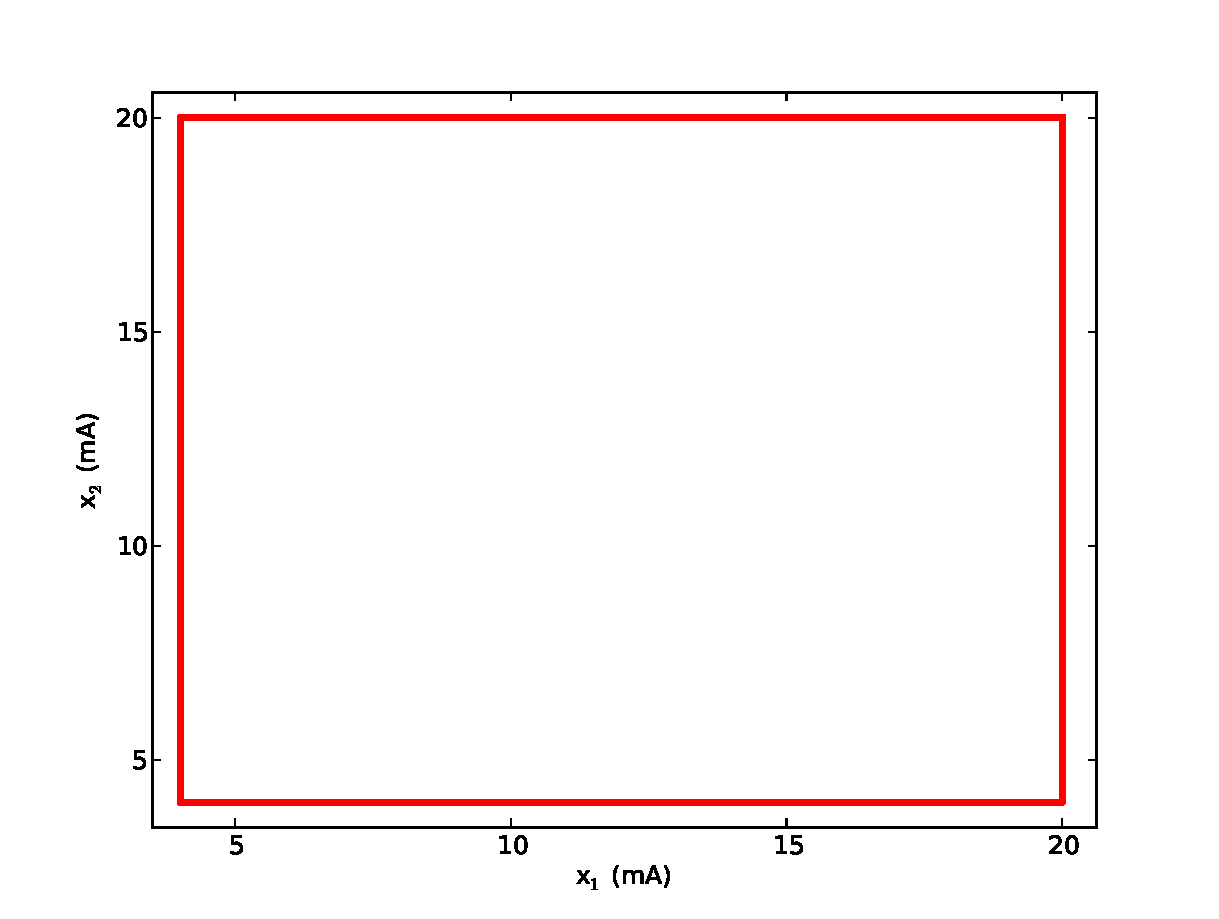
\includegraphics[width=7cm]{graph/flowais.pdf}
    \qquad
    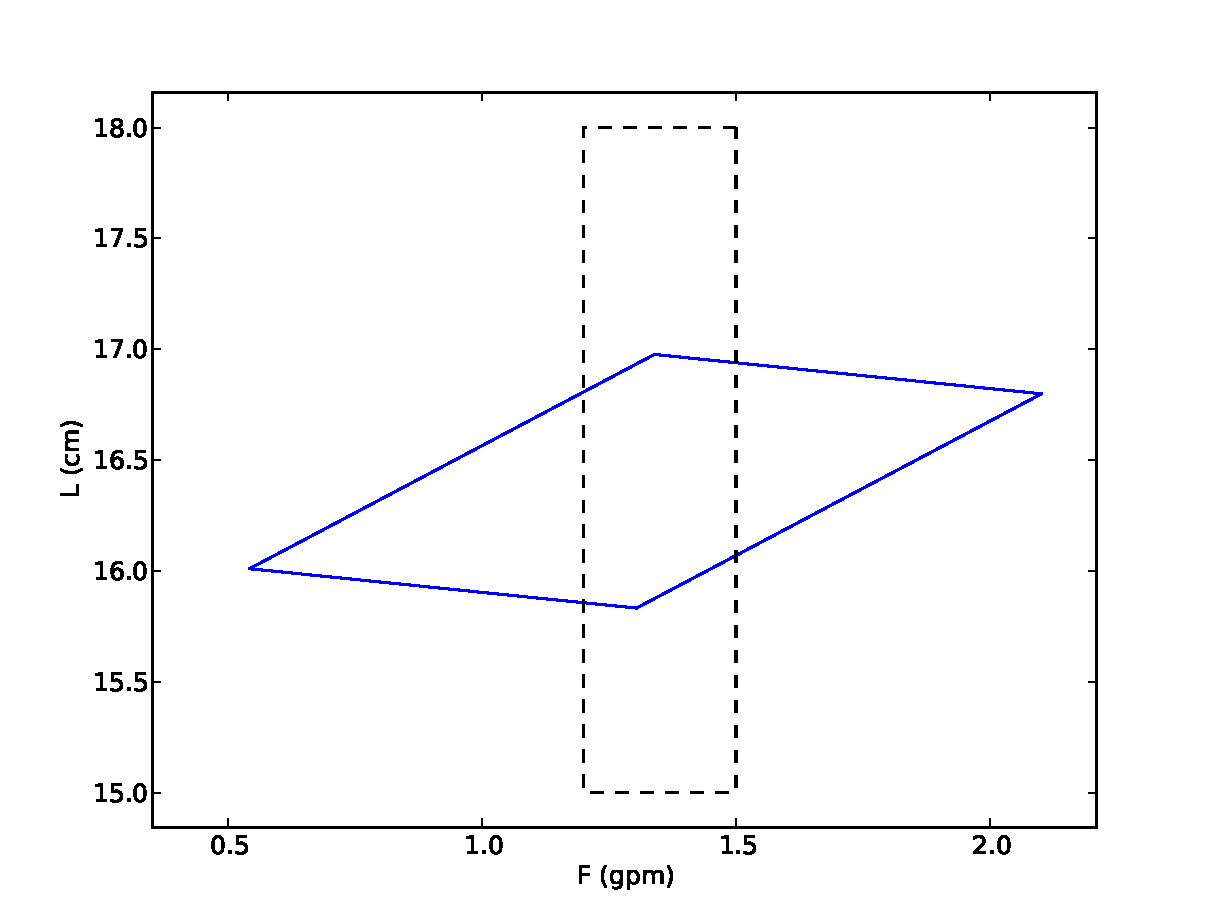
\includegraphics[width=7cm]{graph/flowaos.pdf}
  \caption[AIS, AOS and DOS of the level and flow rig]{AIS (left), AOS and DOS (right) for the level and flow rig.}
  \label{fig:flowaisaos}
\end{figure}

\subsubsection{Set fitting}
It is clear that the level range expectations of this process is too ambitious.
Decreasing these limits will not affect the control adversely, as the model suggests that these upper and lower level limits are not attainable.
Figure~\ref{fig:flowfitbox} shows the fitting of upper/lower constraints within the intersection of the AOS and the DOS.
The dark box represents the largest operating region (described only by high/low limits on the outputs) which are within the original DOS and the AOS.
This procedure increases the OI to 1 and presents tighter bounds that are all feasible.

\begin{figure}[htbp]
  \centering
    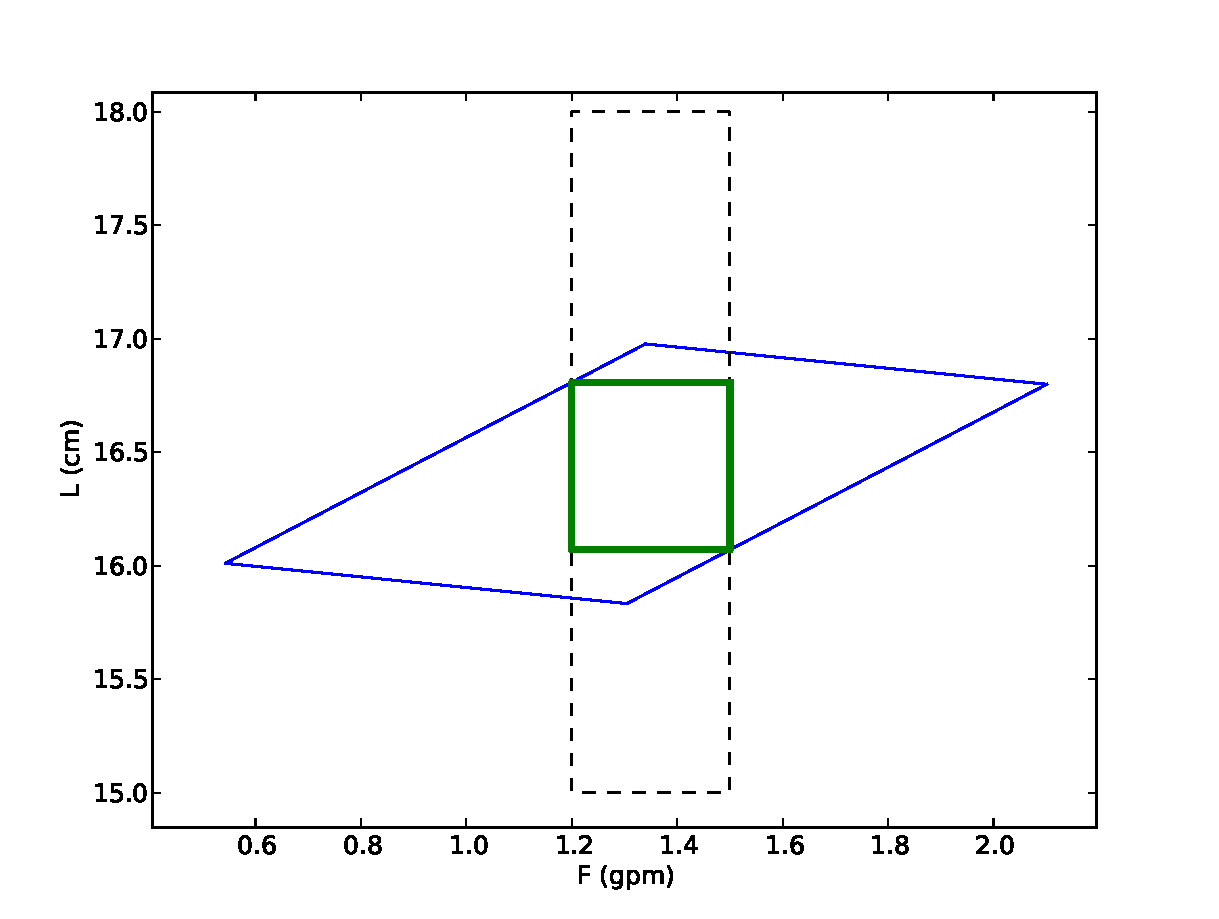
\includegraphics[width=8cm]{graph/flowfitbox.pdf}
  \caption{Fitted high/low constraints in the AOS/DOS intersection.}
  \label{fig:flowfitbox}
\end{figure}
\subsubsection{Feasibility}
\subsubsection{Constraint types}
\subsubsection{Constraint changes}
\subsubsection{MPC interfacing}

\subsection{Laboratory distillation column}
\subsubsection{Input/Output spaces}
From the data in table~\ref{tab:columnopcon} and equation~\ref{eq:columnmodel} the AIS and AOS of the laboratory distillation column can be generated as shown in figure~\ref{fig:columnaisaos}.
Take note that the operating limits for $R$ is used to construct the AIS as values outside of this range (although) possible cause the validity of the model to diminish.
The DOS, as described by the operating range in table~\ref{tab:columnopcon}, is also shown.

\begin{figure}[htbp]
  \centering
    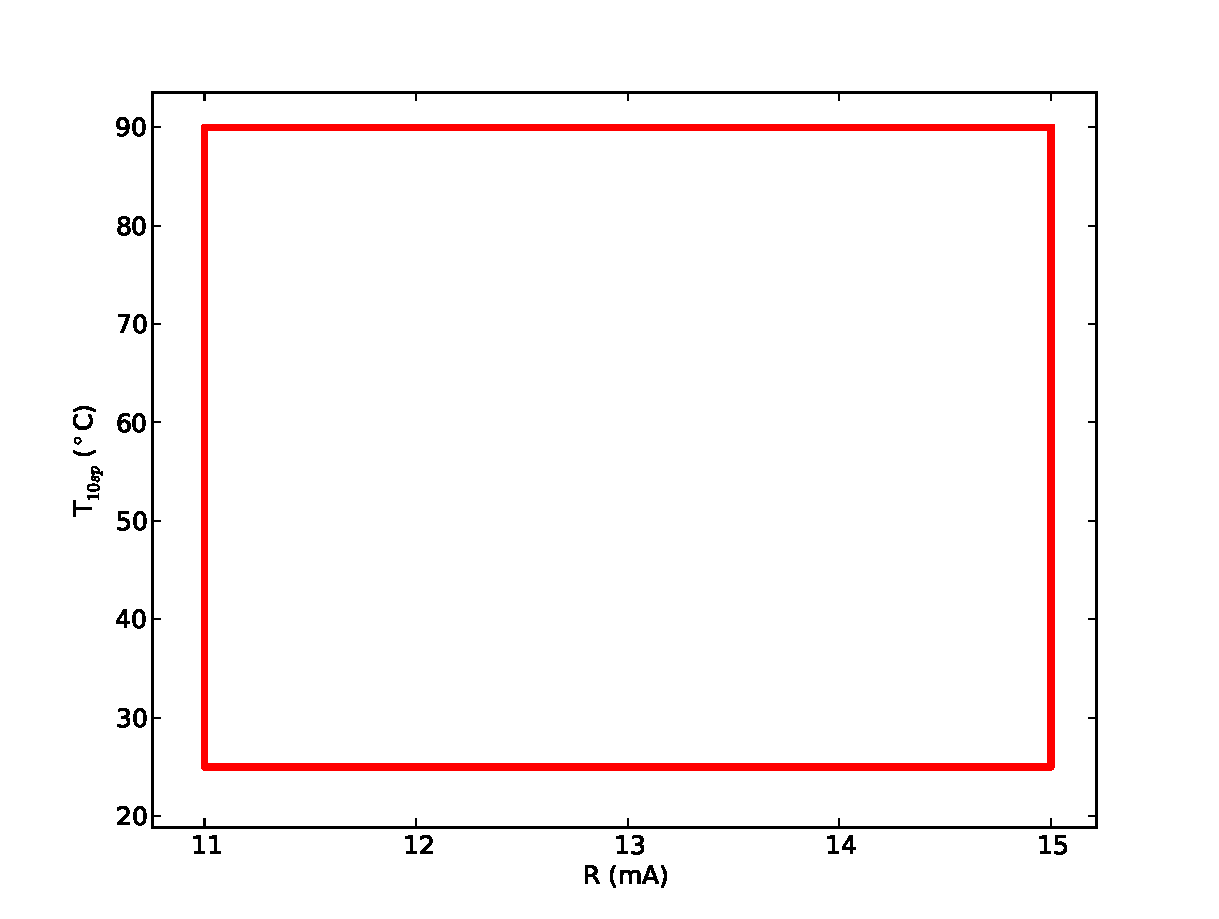
\includegraphics[width=7cm]{graph/columnais.pdf}
    \qquad
    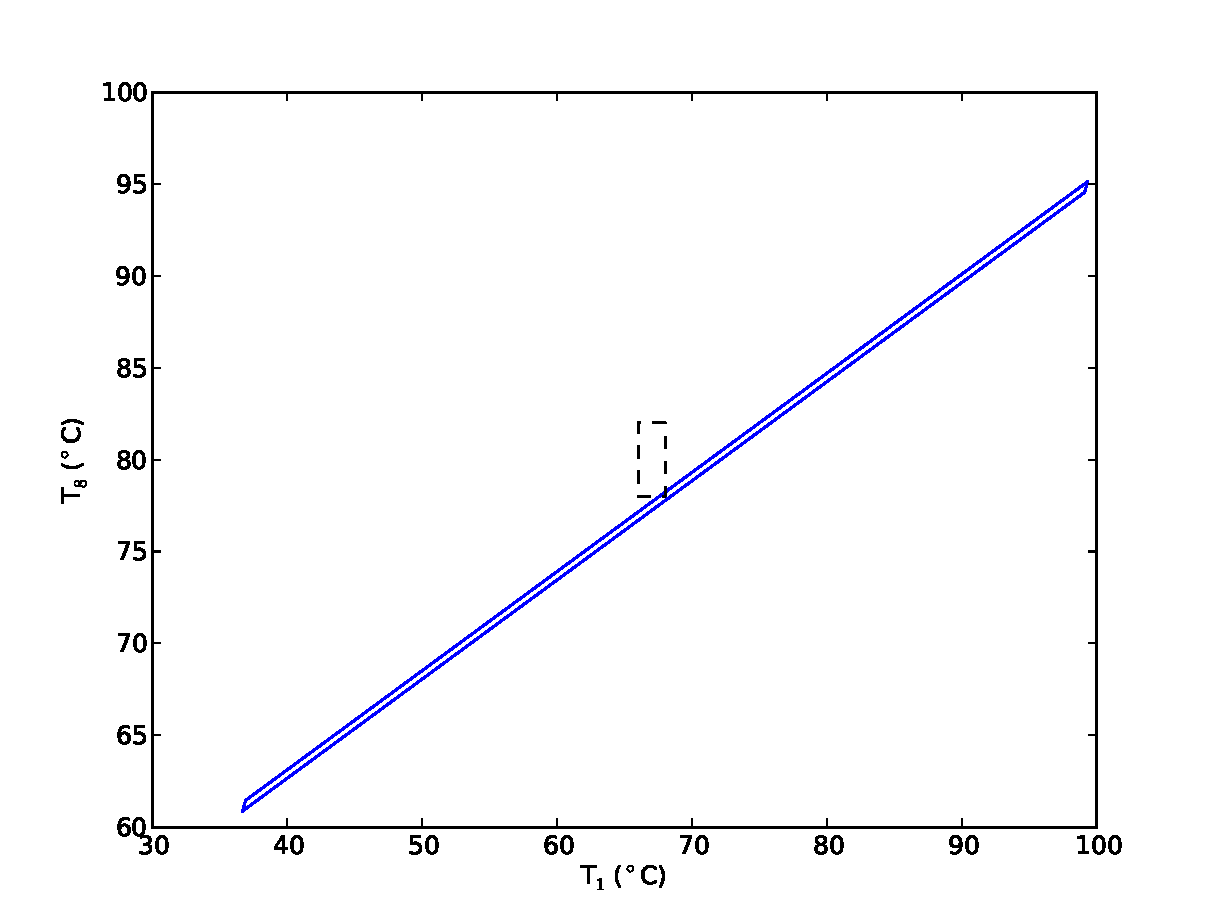
\includegraphics[width=7cm]{graph/columnaos.pdf}
  \caption[AIS, AOS and DOS of the laboratory distillation column]{AIS (left), AOS and DOS (right) of the laboratory distillation column.}
  \label{fig:columnaisaos}
\end{figure}

Figure~\ref{fig:columnaosfocus} focuses on the intersection of the AOS and the DOS.
The calculated OI is 0.006 which confirms that only a very small operating region within the DOS is attainable.
It is also clear that the upper limit of 82$\degrees{C}$ on $T_8$ is unrealistic as the maximum value of $T_8$ (in the operating region) is only 78.2$\degrees{C}$.

\begin{figure}[htbp]
  \centering
    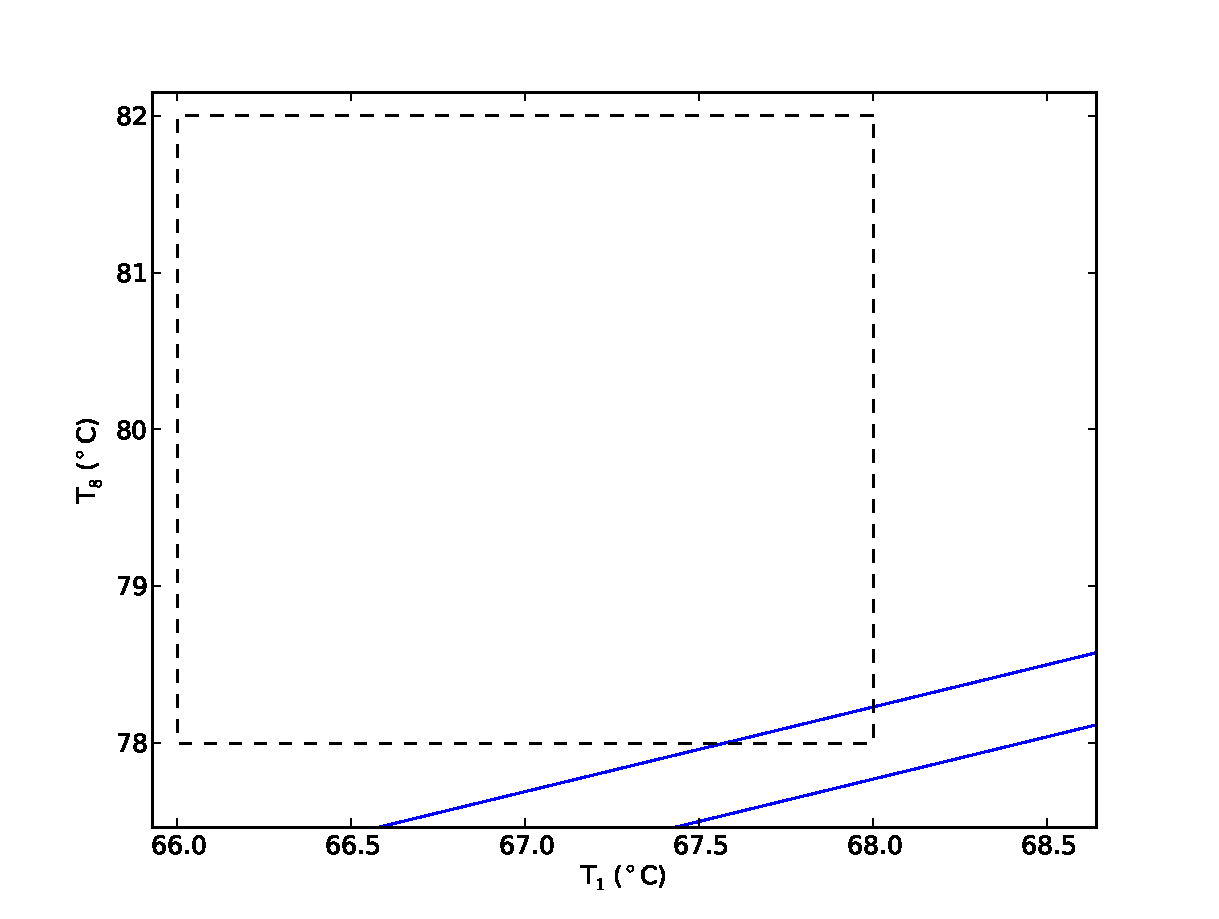
\includegraphics[width=8cm]{graph/columnaosfocus.pdf}
  \caption[AOS and DOS intersection of the laboratory distillation column]{The AOS and DOS intersection shows a very small operating region.}
  \label{fig:columnaosfocus}
\end{figure}

\subsubsection{Set fitting}
\subsubsection{Constraint reformatting}
\subsubsection{Constraint types}
\subsubsection{MPC interfacing}

\section{Constraint set fitting}
The fitting of constraint sets, which form a large part of this dissertation, is discussed separately.
Observations made whilst studying the fitting of constraint sets, which could lead to future research is discussed in section~\ref{sec:setfitfuture}.

\subsection{Solution times}
The use of constrained, gradient-based solvers proved to be significantly faster than unconstrained solvers.
Inconsistent gradient information does, however, hamper their use.

Figure~\ref{fig:cubefittime} compares the solution times of SLSQP and simplex for rectangular set fitting.
Arbitrary sets with three constraints on two variables were generated and a high/low constraint set on the two variables were fitted.

\begin{figure}[htbp]
  \centering
    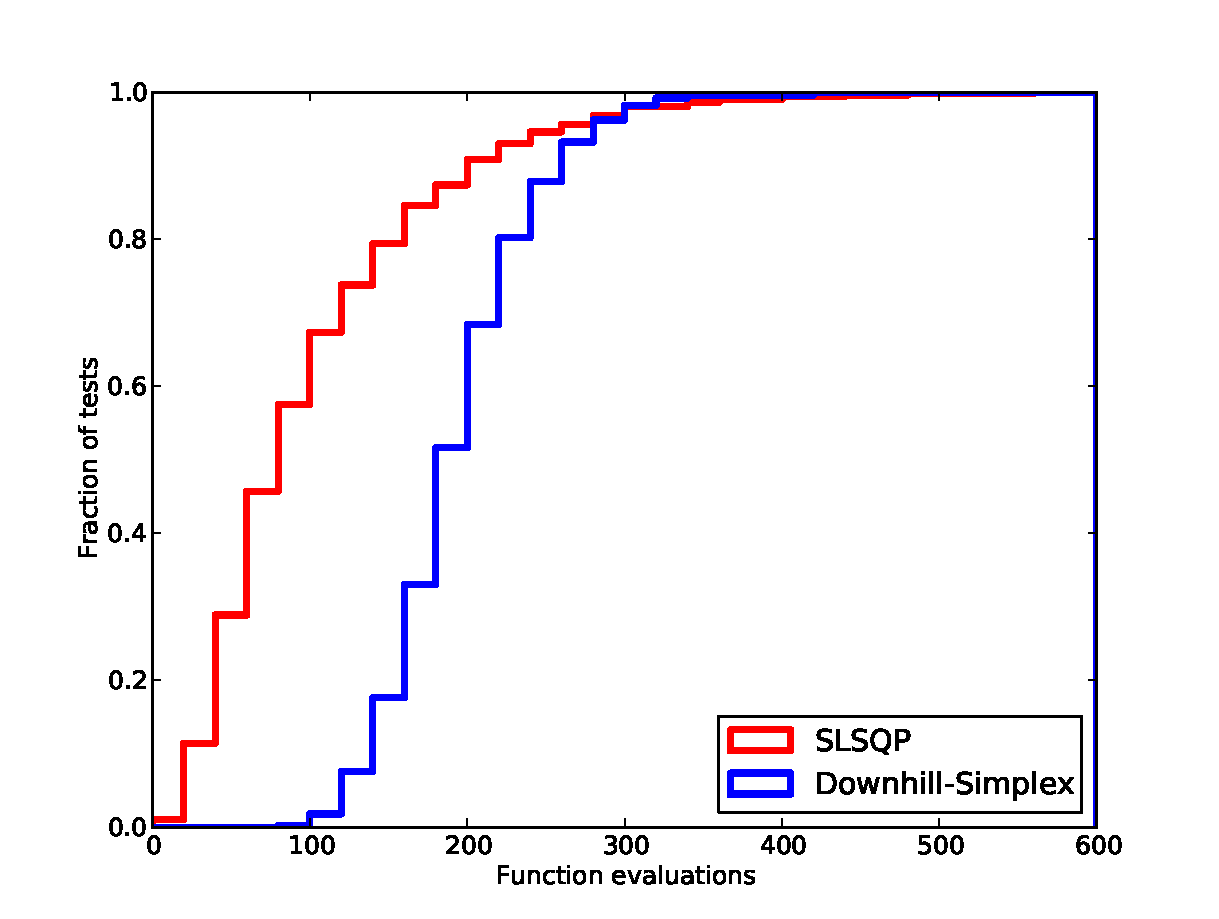
\includegraphics[width=8cm]{graph/cubefittime}
  \caption[SLSQP and simplex calculation time comparison]{Cumulative plot of function evaluations showing faster execution of SLSQP vs simplex}
  \label{fig:cubefittime}
\end{figure}

Fitting a constraint set of an arbitrary size was unsuccessful using constrained, gradient-based solvers.
Possible reasons for this is inconsistent gradient information regarding the position of vertices outside the initial set and the superfluous degrees of freedom present in the problem formulation.

\subsection{Accuracy}
The solutions for high/low constraint set fitting resulted in an optimal answer for each test.
The fitting of arbitrary sized constraint sets suffered from accuracy issues due to the high dependence on the starting point.
As mentioned in the preceding section, due to problems with the unconstrained, gradient-based solvers, only simplex was used for the fitting of arbitrary sets.

\subsubsection{Two variable systems}\label{sec:2dfitting}
For these tests, a 3-constraint set was fitted into a 4-constraint set.
The initial set was chosen to be rectangular (high/low limits) to enable the algebraic calculation of the optimal fitted set.
The optimal solution is 50\% of the volume (area in 2 dimensions) of the initial constraint set.
Figure~\ref{fig:arbfitaccuracy2d} shows the accuracy of this fitting test.
It can be seen that 80\% of the solutions were within 10\% of the optimal solution.
\begin{figure}[htbp]
  \centering
    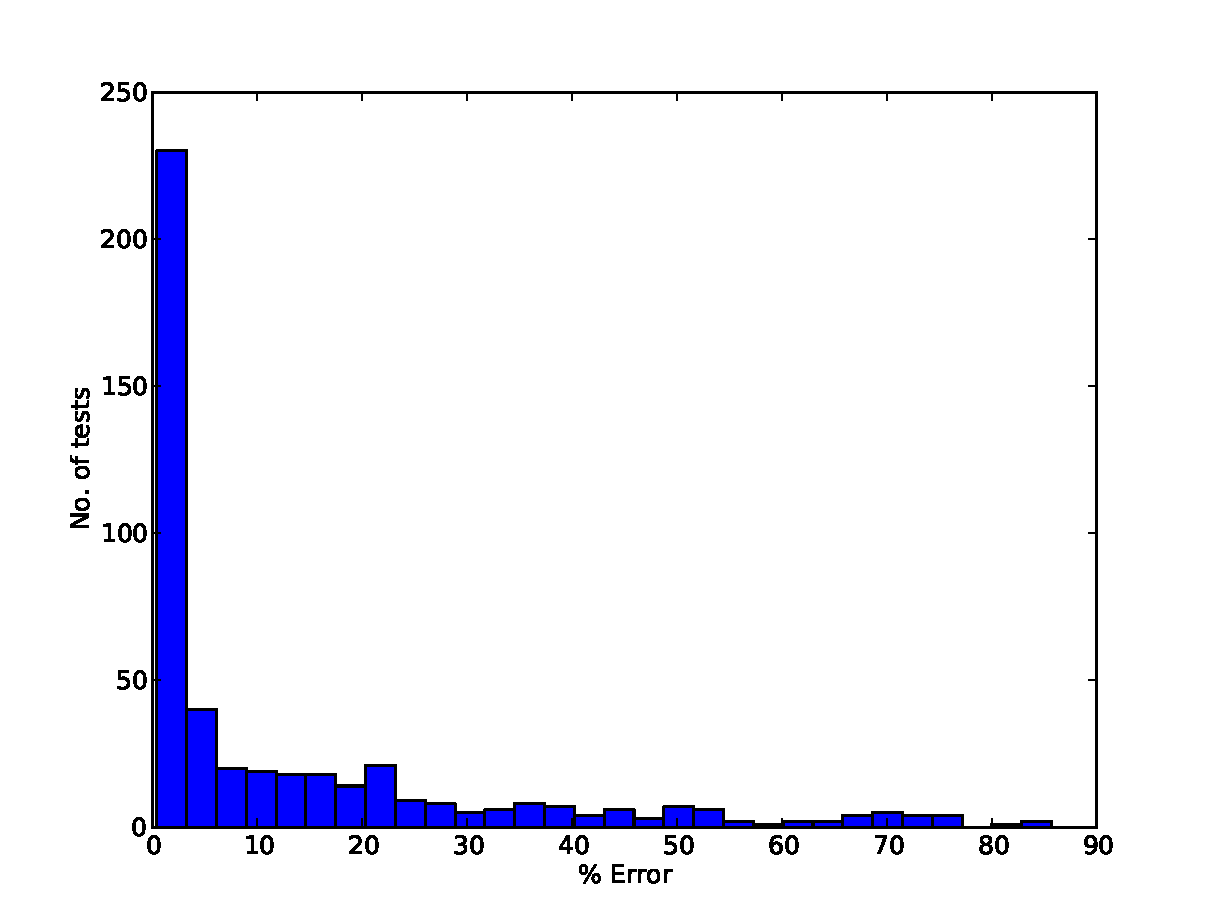
\includegraphics[width=8cm]{graph/arbfitaccuracy2d.pdf}
  \caption[Accuracy of constraint set fitting for 2 variables]{Accuracy of fitting results for a 3-constraint set into a 4-constraint set.}
  \label{fig:arbfitaccuracy2d}
\end{figure}

To increase the accuracy, a multi-start approach was taken where 25 random starting points are generated.
The largest volume set (of the 25 generated) was then used for the fitting.
Figure~\ref{fig:arbfitaccuracy2dmulti} shows the improvement in accuracy with this method.

\begin{figure}[htbp]
  \centering
    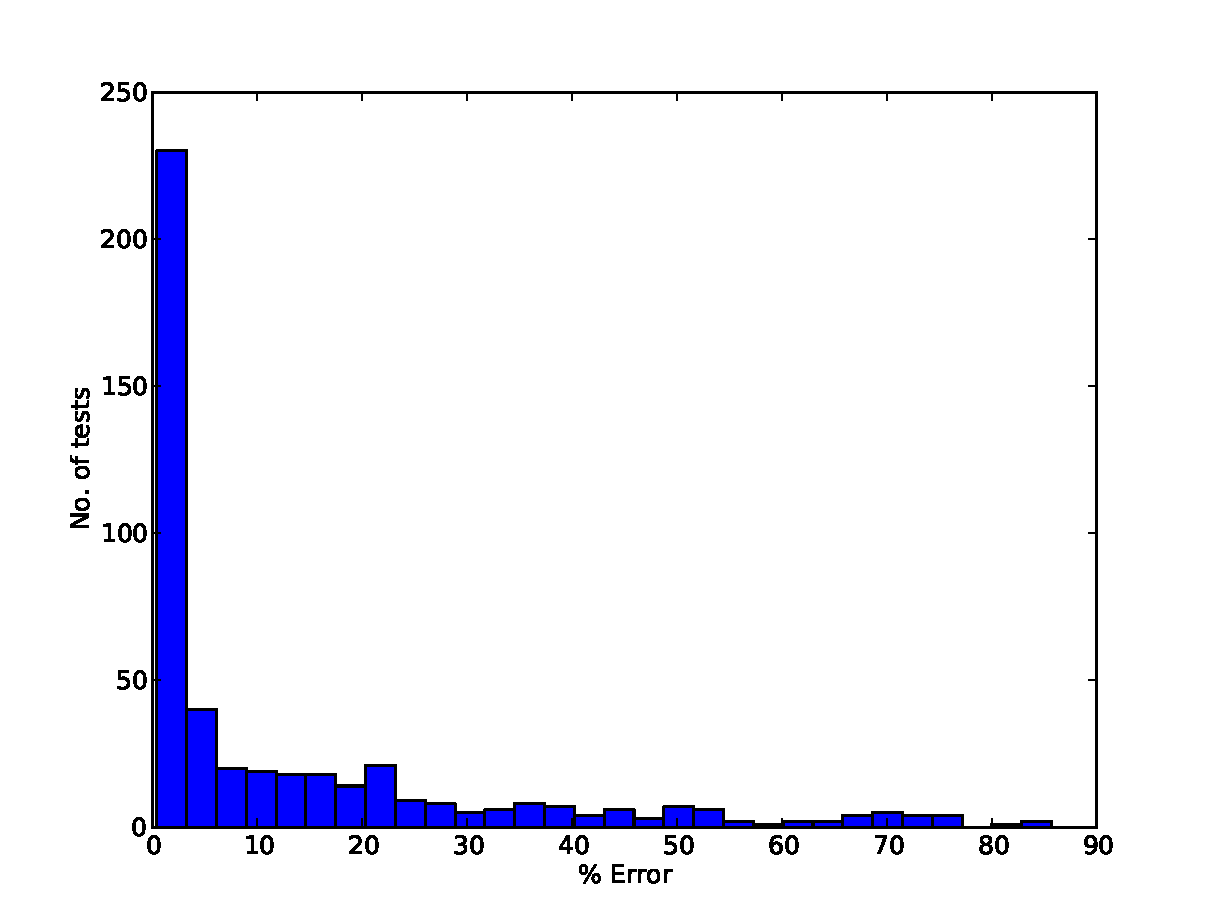
\includegraphics[width=8cm]{graph/arbfitaccuracy2d.pdf}
  \caption[Accuracy of constraint set fitting for 2 variables (multi-start)]{Accuracy increase from the fitting results in figure~\ref{fig:arbfitaccuracy2d} when using a multi-start approach.}
  \label{fig:arbfitaccuracy2dmulti}
\end{figure}
% REPLACE WITH REAL FIGURE

\subsubsection{Three variable systems}
For the three variable tests, a 4-constraint set was fitted into a 6-constraint set.
The initial constraint set was chosen to be a 3-dimensional cube -- again to allow for calculation of the optimal solution.
This test (in geometric terms) results in fitting a tetrahedron into a cube; the optimal solution is 33.33\% of the volume of the cube.
Figure~\ref{fig:arbfitaccuracy3d} shows the accuracy of this test.

\begin{figure}[htbp]
  \centering
    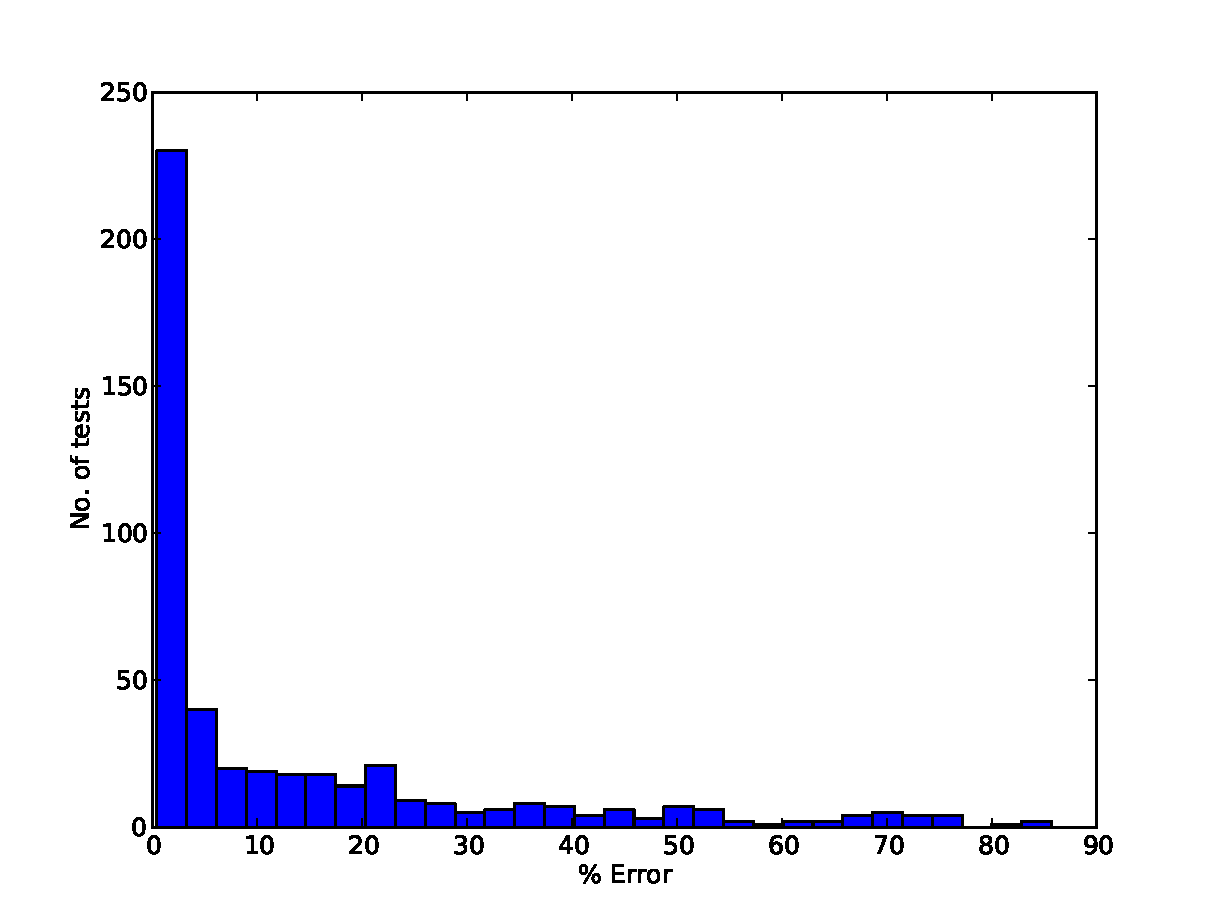
\includegraphics[width=8cm]{graph/arbfitaccuracy2d.pdf}  
  \caption[Accuracy of constraint set fitting for 3 variables]{Low accuracy is obtained for higher dimensional fitting of constraint sets.}
  \label{fig:arbfitaccuracy3d}
\end{figure}

The low accuracy (even when using a multi-start approach) can be ascribed to the increased degrees of freedom and the ill conditioning of the problem.

\subsection{Set fitting expansion}\label{sec:setfitfuture}
The graphs shown in figure~\ref{fig:equaloifits} show a few optimal solutions obtained from the tests of section~\ref{sec:2dfitting}.
It can be noted that even though the sets are not equal, the output operability index \citep{vinsonphd} calculated for all of them are equal.
\begin{figure}[htbp]
  \centering
    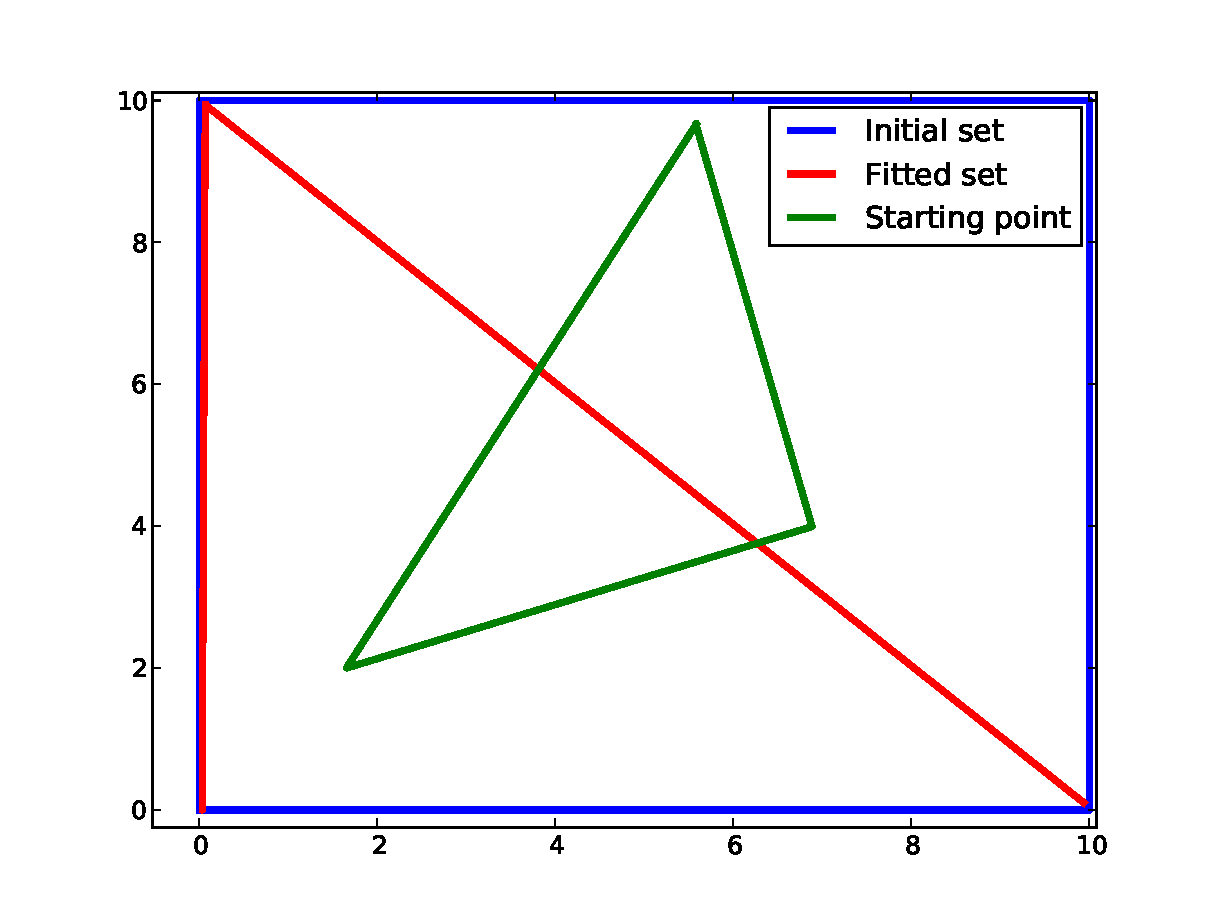
\includegraphics[width=7cm]{graph/2dfit1.pdf}
    \qquad
    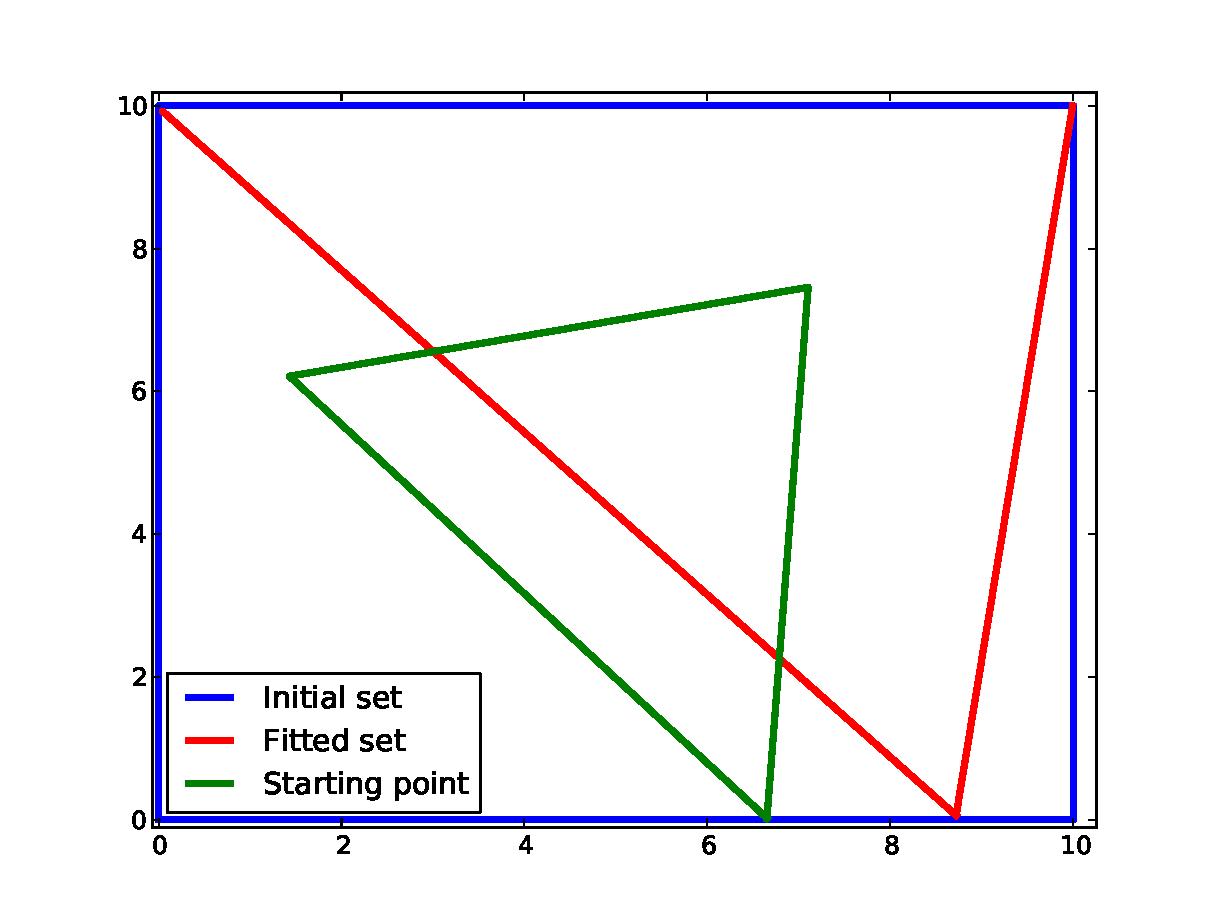
\includegraphics[width=7cm]{graph/2dfit2.pdf}
  \caption[Equal size constraint set fits]{Different sets fitted with an equal size and equal calculated Operability Index.}
  \label{fig:equaloifits}
\end{figure}

From these results the following observations regarding the operability index of \citet{vinsonphd} can be made;
\begin{itemize}
\item the Operability Index is a measure of 'moveability' and emphasises the need for inputs to have a good working range to achieve outputs.
\item all of the input and output space are of equal importance to the Operability Index.
\end{itemize}

It is intuitive that certain sections of the input/output space are of greater importance when considering process economics, sensitivities, etc..
It would therefore be a sensible approach to take into consideration an additional objective function when fitting constraint sets (or when making any changes to the input/output spaces).
Fitting a set as the volume integral of the following possible objective functions would be favourable;
\begin{itemize}
\item Economic objective functions would generate an operating region that maximises profit / minimises cost.
\item Sensitivity functions would identify regions that are problematic to control in and favour them less.
\item Design cost functions would aid in process design when processes are being designed or modified -- costs can be directly related to the improvement in control.
\end{itemize}
These improvements to the constraint set fitting are suggested as a topic for future research.

% Local Variables:
% TeX-master: "AHC_thesis"
% End: